\documentclass[12pt, twoside]{article}
\usepackage[letterpaper, margin=1in, headsep=0.5in]{geometry}
\usepackage[english]{babel}
\usepackage[utf8]{inputenc}
\usepackage{amsmath}
\usepackage{amsfonts}
\usepackage{amssymb}
\usepackage{tikz}
\usepackage{yhmath}
%\usetikzlibrary{quotes, angles}

\usepackage{graphicx}
\usepackage{enumitem}
\usepackage{multicol}

\usepackage{fancyhdr}
\pagestyle{fancy}
\fancyhf{}
\renewcommand{\headrulewidth}{0pt} % disable the underline of the header

\fancyhead[RE]{\thepage}
\fancyhead[RO]{\thepage \\ Name: \hspace{3cm}}
\fancyhead[L]{BECA / Dr. Huson / 10th Grade Geometry\\* 24 May 2019}

\begin{document}
\subsubsection*{11.4 Exam: Quadrilaterals, volume, density, trigonometry, \& review}
 \begin{enumerate}

   \item Given parallelogram $ABCD$ with $m\angle A=55^\circ$, $AB=8$, and $BC=5$. Find the value of each angle measure and side length.
   \begin{multicols}{2}
     \begin{enumerate}
       \item $m\angle B=$\vspace{0.5cm}
       \item $m\angle C=$\vspace{0.5cm}
       \item $m\angle D=$\vspace{0.5cm}
       \item $CD=$ \vspace{0.5cm}
       \item $AD=$ \vspace{0.5cm}
     \end{enumerate}
     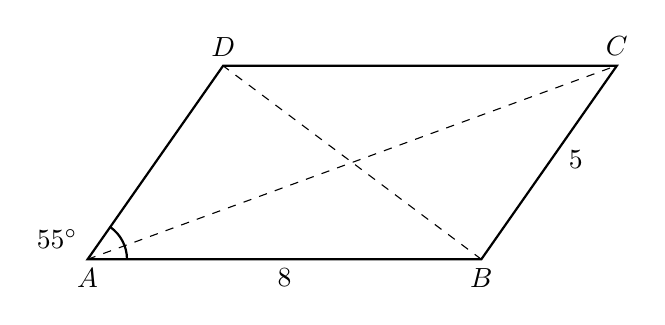
\begin{tikzpicture}[scale=1]
       \draw [thick] (0,0)node[above left]{$55^\circ$}--(5,0)--++(55:3)--(55:3)--cycle;
       \draw [thick] (0.5,0) arc [start angle=0, end angle=55, radius=0.5];
       \draw [dashed] (0,0)node[below]{$A$}--(6.72,2.46)node[above]{$C$};
       \draw [dashed] (5,0)node[below]{$B$}--(55:3)node[above]{$D$};
       \node at (2.5,0)[below]{$8$};
       \node at (6.2,1.5)[below]{$5$};
     \end{tikzpicture}
   \end{multicols} \vspace{1cm}

  \item Circle Always, Sometimes, Never, as applies.
    \begin{center}
      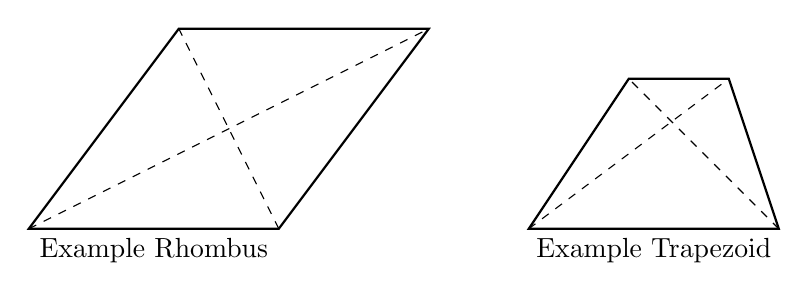
\begin{tikzpicture}[scale=.635]
        \draw [thick] (-2,0) -- (3,0)--(6,4)--(1,4)--cycle;
        \draw [dashed] (-2,0)--(6,4);
        \draw [dashed] (3,0)--(1,4);
        \node at (0.5,0)[below]{Example Rhombus};

        \draw [thick] (8,0) -- (13,0)--(12,3)--(10,3)--cycle;
        \draw [dashed] (8,0)--(12,3);
        \draw [dashed] (13,0)--(10,3);
        \node at (10.5,0)[below]{Example Trapezoid};
      \end{tikzpicture}
    \end{center}
      \begin{enumerate}
        \item Always \quad Sometimes \quad  Never \quad Opposite sides of a parallelogram are congruent. \vspace{0.25cm}
        \item Always \quad Sometimes \quad  Never \quad Diagonals of a rhombus are congruent. \vspace{0.25cm}
        \item Always \quad Sometimes \quad  Never \quad One pair of opposite sides of a trapezoid are congruent. \vspace{0.25cm}
        \item Always \quad Sometimes \quad  Never \quad Adjacent angles of a parallelogram are supplementary.
        \item Always \quad Sometimes \quad  Never \quad At most one pair of sides of a rhombus are congruent. \vspace{0.25cm}
        \item Always \quad Sometimes \quad  Never \quad Diagonals bisect the vertex angles of a rhombus. \vspace{0.25cm}
      \end{enumerate}

\newpage
   \item Three of the vertices of the parallelogram $JKLM$ are given: $J(-3, -2)$, $K(6,1)$, $L(8,5)$. Determine and state the coordinates of the fourth vertex, $M$, and mark and label it on the grid below. Draw the sides of the parallelogram.
     \begin{center}
       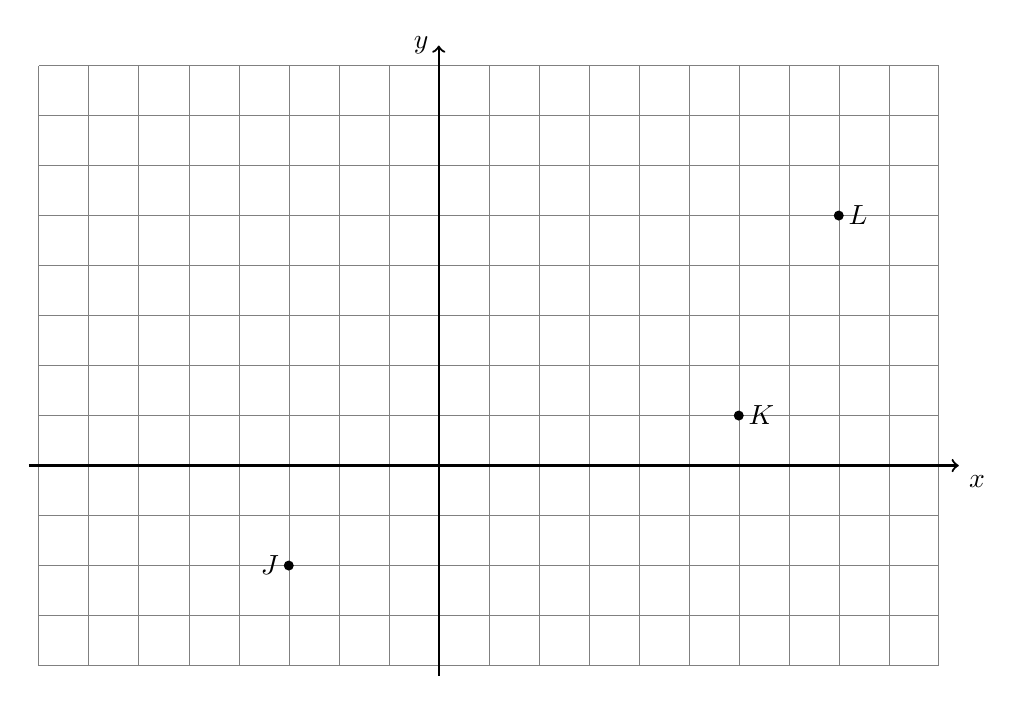
\begin{tikzpicture}[scale=.635]
         \draw [help lines] (-8,-4) grid (10,8);
         \draw [thick, ->] (-8.2,0) -- (10.4,0) node [below right] {$x$};
         \draw [thick, ->] (0,-4.2)--(0,8.4) node [left] {$y$};
         \fill (-3,-2) circle[radius=0.1cm] node[left]{$J$};
         \fill (6,1) circle[radius=0.1cm] node[right]{$K$};
         \fill (8,5) circle[radius=0.1cm] node[right]{$L$};
         %\fill (-1,2) circle[radius=0.1cm] node[right]{$M$};
       \end{tikzpicture}
     \end{center}

  \item A trapezoid has a longer base of 6 and shorter base of 4. One side is perpendicular to the base, and the other is at an angle, as shown. Its height is 3. \\[0.25cm]
    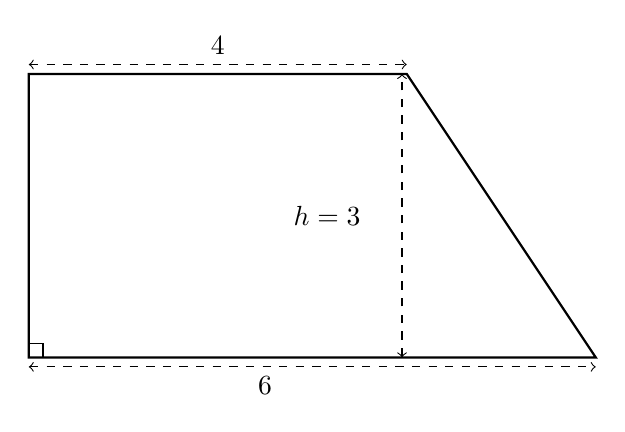
\begin{tikzpicture}[scale=1.2]
     \draw [thick]
     (0,0)--(0,3)--(4,3)--(6,0)--cycle;
     \draw [dashed,<->] (3.95,0)--(3.95,3);
     \draw [dashed,<->] (0,3.1)--(4,3.1);
     %\draw [->] (45:0.5)--(45:0.9142);
     %\draw [->] (45:2.3)--(45:1.9142);
     \draw (0,0)++(0,0.15)--++(0.15,0)--+(0,-0.15);
     \draw [dashed,<->] (0,-0.1)--(6,-0.1);
     \node at (2.5,-0.1)[below]{$6$};
     \node at (2.7,1.5)[right]{$h=3$};
     \node at (2,3.1)[above]{$4$};
    \end{tikzpicture} \vspace{0.25cm}\\
    Determine and state the area of the trapezoid. \vspace{4cm}

\newpage

  \item Draw quadrilateral $ABCD$ with vertices $A(-1, 2)$, $B(5,0)$, $C(8,3)$, and $D(2,5)$ on the grid below. Prove that $ABCD$ is a parallelogram by using slopes to show $\overline{AB} || \overline{CD}$ and $\overline{AD} || \overline{BC}$. \\[0.25cm]
  Calculate the slopes.
  \begin{flushright}
    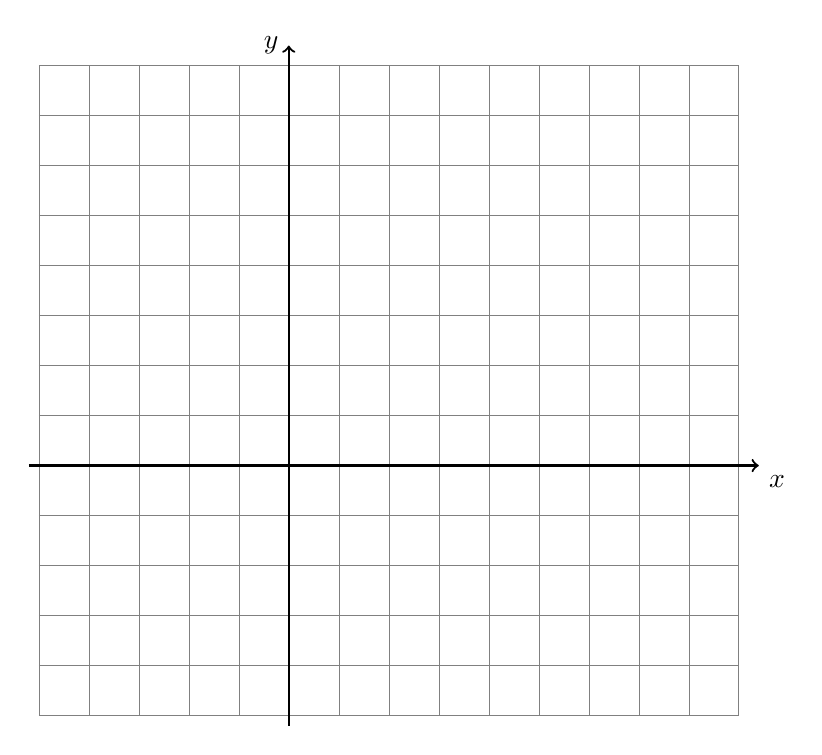
\begin{tikzpicture}[scale=.635]
      \draw [help lines] (-5,-5) grid (9,8);
      \draw [thick, ->] (-5.2,0) -- (9.4,0) node [below right] {$x$};
      \draw [thick, ->] (0,-5.2)--(0,8.4) node [left] {$y$};
    \end{tikzpicture}
  \end{flushright} \vspace{3cm}
    State what slopes are equal to each other, and therefore, what sides are parallel.\\[4cm]
    Finish with a concluding statement.\\[1cm]

\newpage

  \item Find the volume of a cone with diameter of $8$ feet and a height of 7 feet, to the \emph{nearest cubic foot}. \vspace{2.5cm}

  \item A box in the shape of a rectangular prism has a volume of 200 cubic centimeters. It's length is 10 cm and width 5 cm. How tall is it? \vspace{3.0cm}

  \item The area of $\triangle ABC$ is $89.6$ square inches. The altitude of the triangle is $12.8$ inches. Find the length of the base $AB$.\\[0.5cm]
    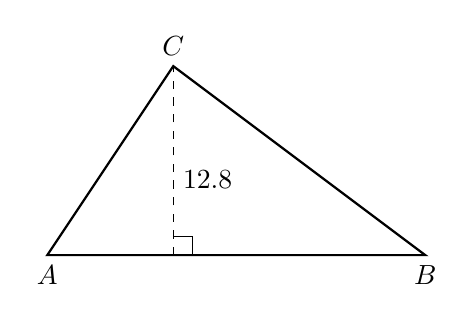
\begin{tikzpicture}[scale=0.8]
     \draw [thick]
       (0,0)node[below]{$A$}--
       (6,0)node[below]{$B$}--
       (2,3)node[above]{$C$} --cycle;
    \draw [dashed] (2,0)--(2,3);
    \draw (2,0)++(0.3,0)--++(0,0.3)--+(-0.3,0);
    \node at (2,1.2)[right]{$12.8$};
    %\node at (3,0)[below]{$20.7$};
  \end{tikzpicture} \vspace{2.25cm}

  \item Find the weight of a steel ball with a diameter of 2.8 inches, to the \emph{nearest tenth of an ounce}. (The density of steel is 4.6 ounce per cubic inch)

\newpage


  \item The long diagonal of rhombus PQRS measures $PR=8$ and the short diagonal is $QS=6$. The intersection of the diagonals is $M$. Find the given measures.\vspace{0.25cm}
    \begin{multicols}{2}
      \begin{enumerate}
        \item $PM=$ \vspace{0.5cm}
        \item $QM=$ \vspace{0.5cm}
        \item $PQ=$ \vspace{0.5cm}
        \item $m\angle SPQ=$\vspace{1.5cm}
      \end{enumerate}
      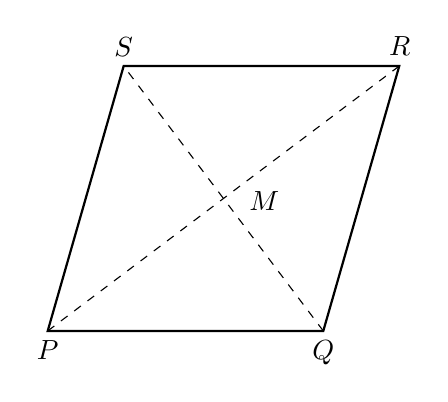
\begin{tikzpicture}[scale=.7]
        \draw [thick] (0,0)--(5,0)--++(74:5)--(74:5)--cycle;
        \draw [dashed] (0,0)node[below]{$P$}--(37:8)node[above]{$R$};
        \draw [dashed] (5,0)node[below]{$Q$}--(74:5)node[above]{$S$};
        \node at (34:4.2)[right]{$M$};
      \end{tikzpicture}
    \end{multicols}
    \vspace{3cm}

  \item A circle with a diameter of 6 in and a central angle of $105^\circ$ is drawn below.
     \begin{enumerate}
       \item What is the area of the sector formed by the $105^\circ$ angle, to the \emph{nearest tenth of a square inch}?\\[0.25cm]
            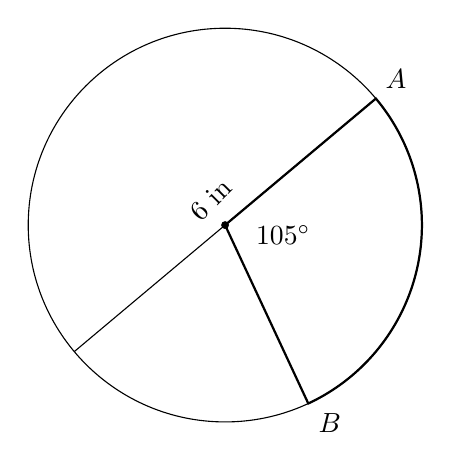
\begin{tikzpicture}[scale=.5]
              \draw (0,0) circle[radius=5];
              \draw (40:5) node[above right]{$A$}--(220:5);
              %\draw (0,0)--(-40:5);
              \fill (0,0) circle[radius=0.1];
              \draw (-10:1.5) node{$105^\circ$};
              \draw (120:0.75) node[rotate=45]{$6$ in};
              \draw [thick] (0,0)--(-65:5)node[below right]{$B$} arc [start angle=-65, end angle=40, radius=5]
              --cycle;
            \end{tikzpicture}
        \vspace{1cm}
       \item What is the length of the arc, $\wideparen{AB}$, to the \emph{nearest tenth of a inch}?
     \end{enumerate}

\newpage

  \item $\triangle ABC$ is shown with $m\angle C=90^\circ$ and the lengths of the triangle's sides are $BC=7$, $AC=8.5$, and $AB=11$.
  \begin{multicols}{2}
        \begin{tikzpicture}[scale=0.7]
          \draw [thick]
          (0,0)node[left]{$A$}--
          (8.5,0)node[ right]{$C$}--
          (8.5,7)node[right]{$B$}--cycle;
          \draw (8.5,0)++(-0.6,0)--++(0,0.6)--+(0.6,0);
          \node at (4,0)[below]{$8.5$};
          \node at (8.5,4)[right]{$7$};
          \node at (3.8,3.5)[above]{$11$};
        \end{tikzpicture}
        \begin{enumerate}
        \item State, as a decimal, the value of $\sin B$. \vspace{1.25cm}
        \item Find the measure of $\angle B$, to the \emph{nearest degree}. \vspace{1.25cm}
        \item Find the degree measure of $\angle A$.
      \end{enumerate}
    \end{multicols}
    \vspace{1.5cm}

  \item Express each trigonometric ratio to the \emph{nearest thousandth} and each angle measure to the nearest degree.
    \begin{multicols}{2}
      \begin{enumerate}
        \item $\sin 42^\circ =$ \vspace{0.5cm}
        \item $\cos^{-1} 0.899 =$ \vspace{0.5cm}
      \end{enumerate}
    \end{multicols} \vspace{0.25cm}

  \item A sailor observes the top of a lighthouse with an angle of elevation of $7^\circ$. She knows the lighthouse is 240 feet tall. Determine and state the distance $x$ between the sailor and the lighthouse, to the \emph{nearest foot}.\\[0.5cm]
    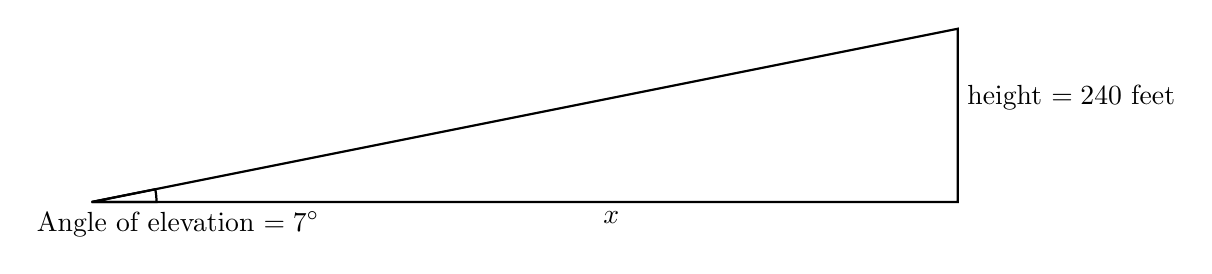
\begin{tikzpicture}[scale=1.1]
     \draw [thick] (10,0)--(0,0)--(10,2.0)--cycle;
     \draw [thick] (0,0)--(0.75,0) arc [start angle=0, end angle=11.3, radius=0.75]--cycle;
     \node at (1,0)[below]{Angle of elevation $=7^\circ$};
     \node at (10,1.2)[right]{height $=240$ feet};
     \node at (6,0)[below]{$x$};
    \end{tikzpicture} \vspace{3.25cm}

\newpage
  \item The line $l$ has the equation $y=-\frac{3}{4}x+3$. To each line below, circle whether $l$ is parallel, perpendicular, or neither.
    \begin{enumerate}
      \item parallel \quad perpendicular \quad neither \qquad $y=\frac{4}{3}x-2$
      \vspace{0.5cm}
      \item parallel \quad perpendicular \quad neither \qquad $y=\frac{3}{4}x+7$
      \vspace{0.5cm}
      \item parallel \quad perpendicular \quad neither \qquad $y=-\frac{3}{4}x +5$
      \vspace{0.5cm}
      \item parallel \quad perpendicular \quad neither \qquad $3x+4y=8$
      \vspace{3.5cm}
    \end{enumerate}

  \item Write an equation of the line that is perpendicular to the line whose equation is $y=\frac{5}{3}x+1$ and passes through the point $(-2,5)$. \vspace{2cm}

  \item Given $m\angle R=31$ and $m\angle U=71$. Find $m\angle UST$.\\[1cm]
  \begin{tikzpicture}
   %\draw [->, thick] (0,0)--(5,5);
   \draw [<-, thick] (8,0)--(0,0)--(3,3)--(4.5,0);
   \draw [fill] (0,0) circle [radius=0.05] node[below]{$R$};
   \draw [fill] (4.5,0) circle [radius=0.05] node[below]{$S$};
   \draw [fill] (3,3) circle [radius=0.05] node[right]{$U$};
   \draw [fill] (7,0) circle [radius=0.05] node[below]{$T$};
  \end{tikzpicture} \vspace{1cm}

  \item Write down the center and radius of each circle, expressing the result as a simplified radical if necessary (not a decimal).
   \begin{enumerate}
     \begin{multicols}{2}
     \item   $(x+1)^2+(y-3)^2=64$ \vspace{2.5cm}
     \item   $x^2+(y-2)^2=18$ \vspace{2.5cm}
     \end{multicols}
   \end{enumerate} \vspace{2cm}

  \newpage
  \item In the diagram below, $\overline{AC}$ has endpoints with coordinates $A(-6,2)$ and $C(6,-2)$.
   \begin{center} %4 quadrant regents grid
     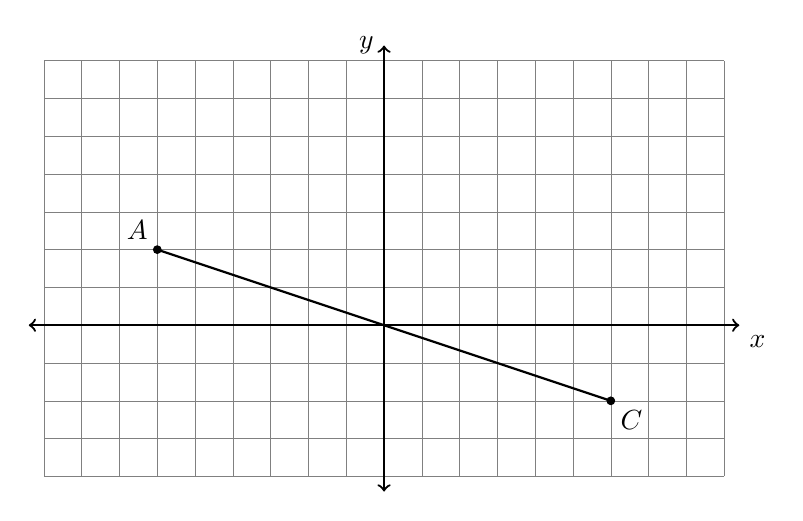
\begin{tikzpicture}[scale=.48]
       \draw [help lines] (-9,-4) grid (9,7);
       \draw [thick, <->] (-9.4,0) -- (9.4,0) node [below right] {$x$};
       \draw [thick, <->] (0,-4.4)--(0,7.4) node [left] {$y$};
       \draw [thick] (-6, 2)--(6,-2);
       \draw [fill] (-6, 2) circle [radius=0.1] node[above left] {$A$};
       \draw [fill] (6, -2) circle [radius=0.1] node[below right] {$C$};
     \end{tikzpicture}
   \end{center}
   If $B$ is a point on $\overline{AC}$ and $AB {:} BC = 1{:}3$,  what  are  the coordinates of $B$? \vspace{4cm}

  \item Triangle $ABC$ is dilated with a scale factor of $k$ centered at $A$, yielding $\triangle ADE$, as shown. Given $AB=9$, $BC=9$, $AC=12$, and $DE=15$. \\[0.25cm] Find $BD$, $AE$, and $k$ (the scale factor).\\[0.25cm]
     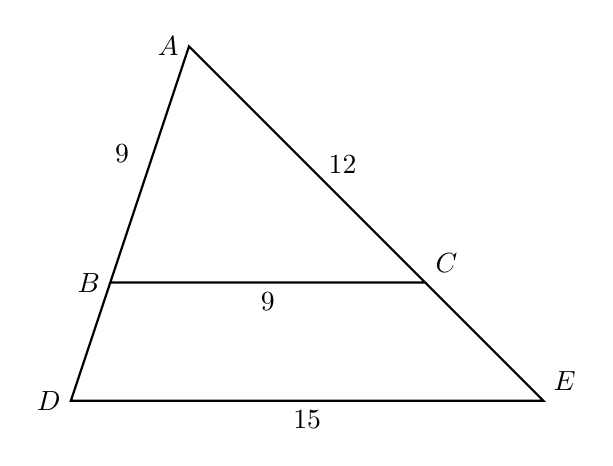
\begin{tikzpicture}[scale=0.5]
       \draw [thick]
       (0,0)node[left]{$B$}--
       (8,0)node[above right]{$C$}--
       (2,6)node[left]{$A$}--cycle;
       \draw [thick]
       (0,0)--
       (-1,-3)node[left]{$D$}--
       (11,-3)node[above right]{$E$}--(8,0);
       \node at (4,0)[below]{$9$};
       \node at (5.3, 3)[right]{$12$};
       \node at (0.3, 2.8)[above]{$9$};
       \node at (5,-3)[below]{$15$};
     \end{tikzpicture}
  \vspace{2cm}

\newpage
  \item What is the smallest non-zero angle of rotation about its center that would map the equilateral triangle onto itself? \vspace{0.25cm}
  \begin{center}
    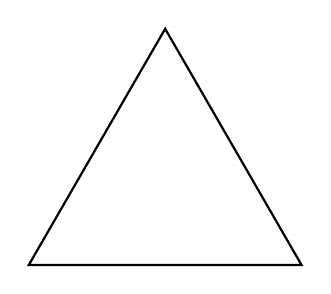
\begin{tikzpicture}%[scale=.48]
      \draw [thick]
      (-30:2)--
      (90:2)--
      (210:2)--cycle;
    \end{tikzpicture}
  \end{center} \vspace{1cm}

  \item A translation maps $A(1,6) \rightarrow A'(-2,4)$. What is the image of $B(4,5)$ under the same translation?  \vspace{2.5cm}

  \item What transformation maps $\triangle ABC$ onto $\triangle DEF$, shown below? Fully specify the transformation.
    \begin{center}
      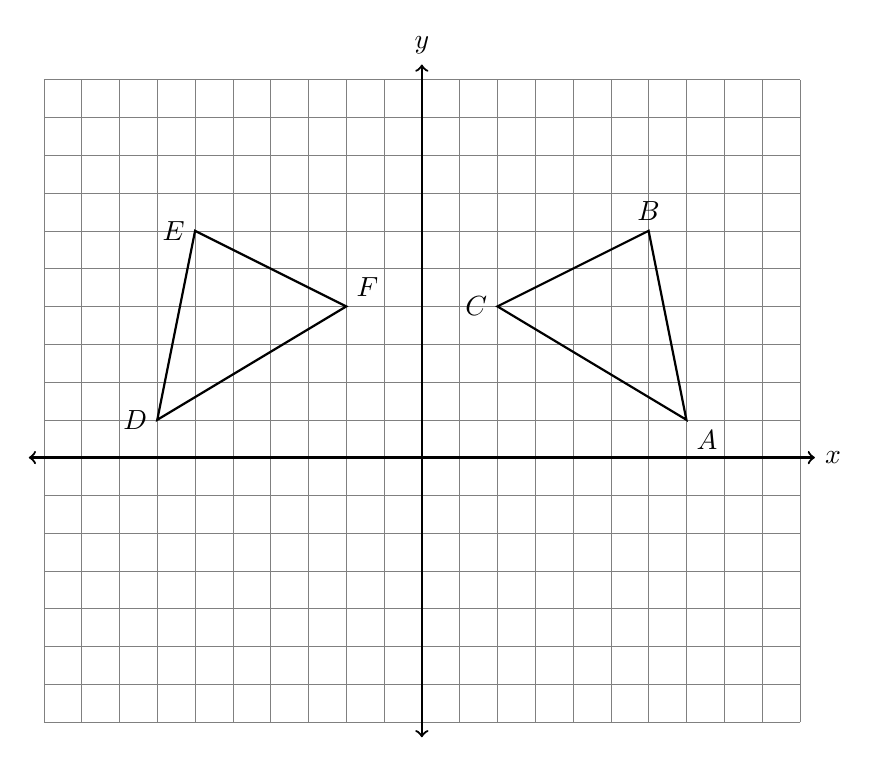
\begin{tikzpicture}[scale=.48]
        \draw [help lines] (-10,-7) grid (10,10);
        \draw [thick, <->] (-10.4,0) -- (10.4,0) node [right] {$x$};
        \draw [thick, <->] (0,-7.4)--(0,10.4) node [above] {$y$};
        \draw [thick]
          (7,1) node[below right] {$A$}--
          (6,6) node[above] {$B$}--
          (2,4) node[left] {$C$}--cycle;
        \draw [thick]
          (-7,1) node[left] {$D$}--
          (-6,6) node[left] {$E$}--
          (-2,4) node[above right] {$F$}--cycle;
      \end{tikzpicture}
    \end{center}

\newpage
  \item Given circle $O$ with inscribed $\triangle AOB$. $m\angle O=100^\circ$. Find $m\angle A$.\\[1cm]
      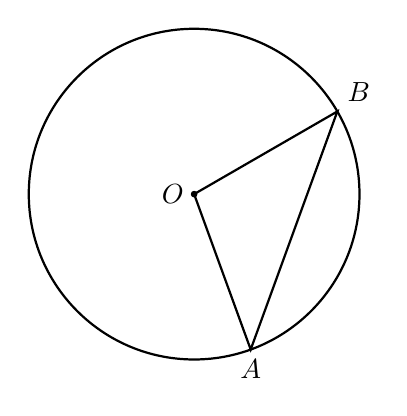
\begin{tikzpicture}[scale=0.7]
        %\draw [-, thick] (-6,0) node[left]{$A$}--(0,0);
        \draw  [thick] (0,0) circle [radius=3] node[left]{$O$};
        \draw [thick] (-70:3) node[below]{$A$}--(0,0)
          --(30:3) node[above right]{$B$}--cycle;
        \draw [fill] (0,0) circle [radius=0.05];
      \end{tikzpicture} \vspace{1cm}

  \item Given circle $P$ with $m \angle APB=70^\circ$.
    \begin{multicols}{2}
     \raggedcolumns
     \begin{enumerate}
       \item Write down the $m \wideparen{AB}$. \vspace{1.7cm}
       \item Find the $m\angle AQB$. \vspace{2cm}
     \end{enumerate}
       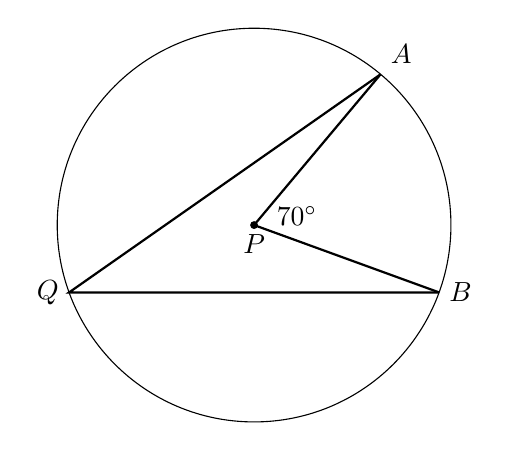
\begin{tikzpicture}[scale=.5]
         \draw (0,0) circle[radius=5];
         \draw [thick]
         (-20:5) node[right] {$B$}--
         (0,0) --
         (50:5) node[above right] {$A$};
         \draw [thick] (-20:5)--(200:5) node[left] {$Q$}--(50:5);
         \draw (35:0.4) node[right]{$70^\circ$};
         \fill (0,0) circle[radius=0.1] node[below]{$P$};
       \end{tikzpicture}
    \end{multicols}

    \item Given circle $O$ with chords $\overline{AD}$ and $\overline{BE}$ intersecting at $C$, as shown in the diagram. Given $m \wideparen{AB}=83^\circ$, $m \wideparen{BD}=74^\circ$, and $m \wideparen{DE}=53^\circ$.
      \begin{multicols}{2}
       \raggedcolumns
       \begin{enumerate}
         \item Find the $m\angle ACB$. \vspace{3.5cm}
         \item Find the measure of the minor arc, $m\wideparen{AE}$. \vspace{2cm}
       \end{enumerate}
       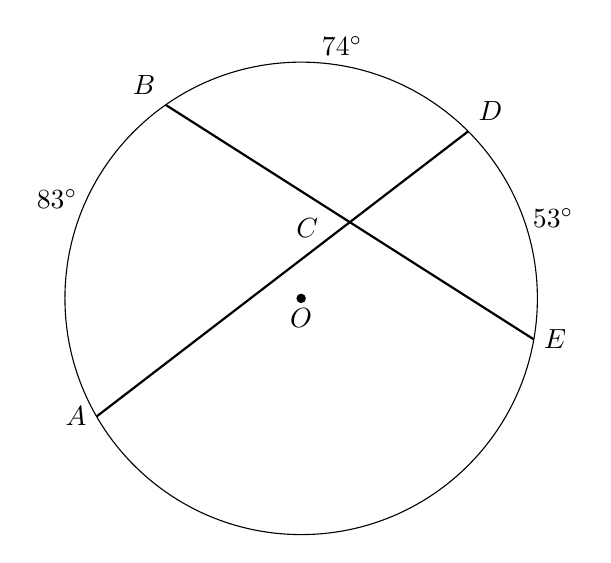
\begin{tikzpicture}[scale=.6]
         \draw (0,0) circle[radius=5];
         \draw [thick]
         (-10:5) node[right] {$E$}--
         (125:5) node[above left] {$B$};
         \draw [thick] (210:5) node[left] {$A$}--
         (45:5) node[above right] {$D$};
         \draw (85:1.5) node{$C$};
         \draw (20:5) node[right] {$53^\circ$};
         \draw (80:5) node[above] {$74^\circ$};
         \draw (155:5) node[left] {$83^\circ$};
        \fill (0,0) circle[radius=0.1] node[below]{$O$};
       \end{tikzpicture}
      \end{multicols}  \vspace{2cm}

\newpage
\subsubsection*{Early finishers}

  \item A monument in the shape of a pyramid with a square base has a volume of 60,750 cubic feet. If its height measures 30 feet, what is the length of the side of the base? \vspace{4cm}

  \item Reflect $\triangle PQR$ across the $x$-axis, drawing its image $\triangle P'Q'R'$ and labeling its vertices.
    \begin{center}
      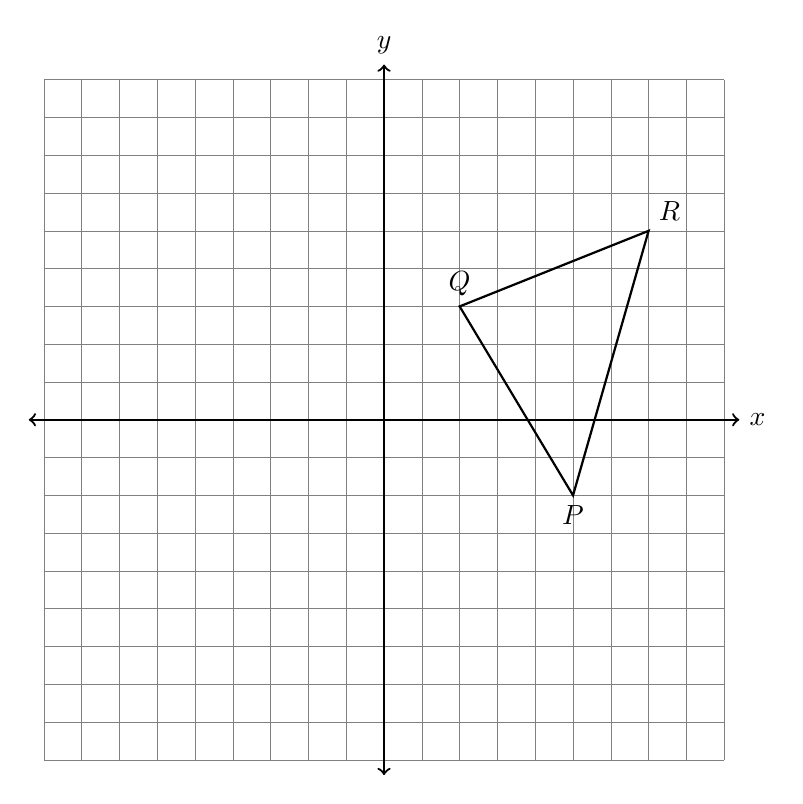
\begin{tikzpicture}[scale=.48]
        \draw [help lines] (-9,-9) grid (9,9);
        \draw [thick, <->] (-9.4,0) -- (9.4,0) node [right] {$x$};
        \draw [thick, <->] (0,-9.4)--(0,9.4) node [above] {$y$};
        \draw [thick]
          (5,-2) node[below] {$P$}--
          (2,3) node[above] {$Q$}--
          (7,5) node[above right] {$R$}--cycle;
      \end{tikzpicture}
    \end{center}


  \item If $\sin (3x+20)^\circ = \cos 25^\circ$, what is the value of $x$? \vspace{3cm}

\newpage
  \item The secants $\overline{ABC}$ and $\overline{ADE}$ intersect the circle $O$, as shown in the diagram. \\Given $m \wideparen{BD}=40^\circ$ and $m \wideparen{CE}=170^\circ$. Find the $m\angle A$.
   \begin{center}
   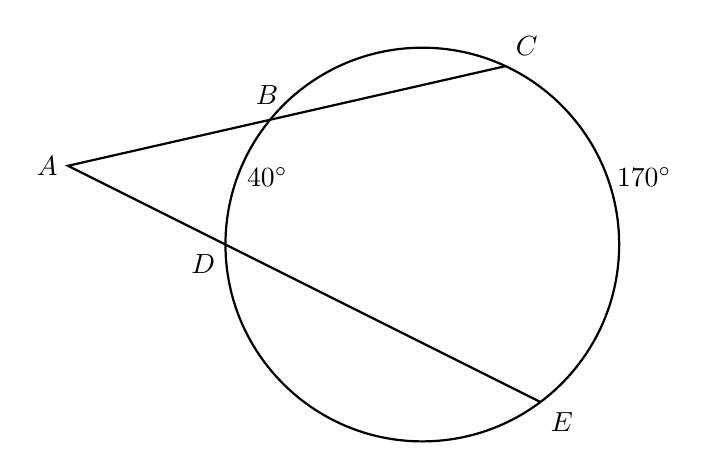
\begin{tikzpicture}[scale=.5]
     \draw [thick] (0,0) circle[radius=5];
     \draw [thick]
     (3,-4) node[below right] {$E$}--
     (-5,0) node[below left] {$D$}--
     (-9,2) node[left] {$A$}--
     (65:5) node[above right] {$C$};
     \draw (132:5.1) node[left] {$B$};
     \draw (20:5) node[right] {$170^\circ$};
     \draw (160:5) node[right] {$40^\circ$};
   \end{tikzpicture}
 \end{center} \vspace{1cm}

  \item A staircase riser is cut as a series of congruent triangles with each step's ``rise" equal to 7.5 inches, and the ``run" of each step is 8.5 inches, as shown below. ($AB=7.5$ and $BC=8.5$)
  \begin{enumerate}
    \item What is the angle of inclination of the staircase, $x$, rounded to the \emph{nearest degree}?\\[0.5cm] 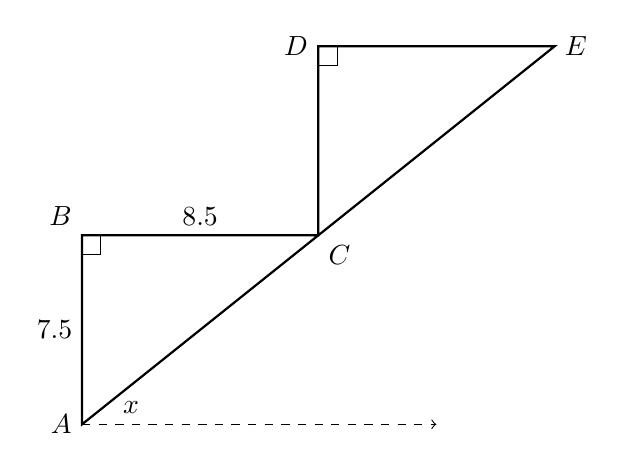
\begin{tikzpicture}[scale=0.3]
          \draw [thick]
          (0,0)node[left]{$A$}--
          (0,8)node[above left]{$B$}--
          (10,8)node[below right]{$C$}--
          (10,16)node[left]{$D$}--
          (20,16)node[right]{$E$}--cycle;
          \draw [dashed, ->] (0,0)--(15,0);
          \draw (0,8)++(0,-0.8)--++(0.8,0)--+(0,0.8);
          \draw (10,16)++(0,-0.8)--++(0.8,0)--+(0,0.8);
          \node at (0,4)[left]{$7.5$};
          \node at (5,8)[above]{$8.5$};
          \node at (28:1.5)[right]{$x$};
        \end{tikzpicture}
      \item Find the diagonal length of the two-step riser, the distance $AE$, to the \emph{nearest tenth of an inch}.
    \end{enumerate} \vspace{2.5cm}


\end{enumerate}
\end{document}

\newpage

  \item On the set of axes below, $\triangle ABC$, altitude $\overline{GC}$, and  median $\overline{MC}$ are drawn.
    \begin{center}
      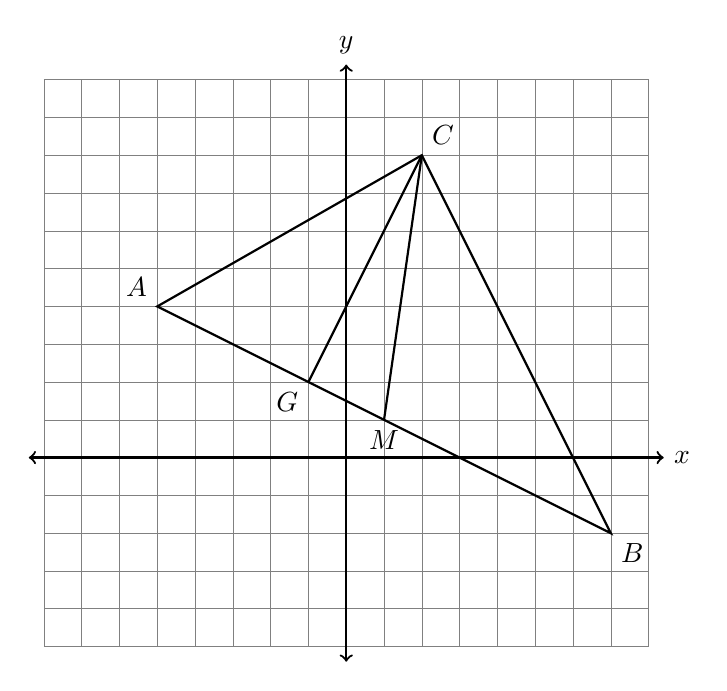
\begin{tikzpicture}[scale=.48]
        \draw [help lines] (-8,-5) grid (8,10);
        \draw [thick, <->] (-8.4,0) -- (8.4,0) node [right] {$x$};
        \draw [thick, <->] (0,-5.4)--(0,10.4) node [above] {$y$};
        \draw [thick]
          (-5,4) node[above left] {$A$}--
          (7,-2) node[below right] {$B$}--
          (2,8) node[above right] {$C$}--
          cycle;
        \draw [thick] (1,1) node[below] {$M$}--(2,8);
        \draw [thick] (-1,2) node[below left] {$G$}--(2,8);
      \end{tikzpicture}
    \end{center}
      Determine which equations represent the area of the triangle, circling True or False.
      \begin{multicols}{2}
       \begin{enumerate}
          \item \quad T \quad F \quad $\displaystyle Area_\triangle = \frac{(CG)(AB)}{2}$
          \item \quad T \quad F \quad $\displaystyle Area_\triangle = \frac{(CM)(AB)}{2}$ \vspace{0.25cm}
          \item \quad T \quad F \quad $\displaystyle Area_\triangle = \frac{(AC)(AB)}{2}$ \vspace{0.25cm}
          \item \quad T \quad F \quad $\displaystyle Area_\triangle = \frac{(CG)(BC)}{2}$
      \end{enumerate}
      \end{multicols}
      \vspace{0.25cm}



        \item The map of a campground is shown below. Campsite C, first aid station F, and supply station S lie along a straight path. The path from the supply station to the tower, T, is perpendicular to the path from the supply station to the campsite. The length of path FS is 400 feet. The angle formed by path TF and path FS is $72^\circ$. The angle formed by path   and path CS is $55^\circ$.\\[0.5cm]
        \includegraphics[width=0.5\textwidth]{camp_Jun2018-31.png}
          \begin{enumerate}
            \item Determine and state the volume of concrete needed, \emph{in cubic feet}. \vspace{1cm}
            \item Sarah can mix her own concrete for \$3.25 per cubic foot. How much money will it cost her to replace the two concrete sections?
        \end{enumerate} \vspace{2.5cm}
